\documentclass[11pt,a4paper,titlepage]{article}

\usepackage{pdflscape}
\usepackage[margin=1in]{geometry}
\usepackage{titling}
\usepackage{graphicx}
\usepackage{titlesec}

\graphicspath{ {./Images/} }

\setcounter{secnumdepth}{4}

\titleformat{\paragraph}
{\normalfont\normalsize\bfseries}{\theparagraph}{1em}{}
\titlespacing*{\paragraph}
{0pt}{3.25ex plus 1ex minus .2ex}{1.5ex plus .2ex}

\begin{document}
%\title{ \huge Functional Requirements for the SAMBUG}

\begin{titlepage}
    \centering
    \vfill
    {\bfseries\Huge
         Functional Requirements for the SAMBUG Project\\
      \hfill\\
         \Large COS301
        \vskip2cm
        
\includegraphics[width=6cm]{sambug} \\

    }    
    \vfill
        Abrie van Aardt 13178840\\
		Werner Mostert 13019695\\
		Kele-ab Tessera 13048423\\
		Keagan Thompson 13023782\\
		Michelle Swanepoel 13066294\\
    
    
    \vfill
    
\includegraphics[width=6cm]{logo} \\
    \textbf{May 2015}
    \vfill
\end{titlepage}
	
%\author
%{     
%	Abrie van Aardt 13178840\\
%	Werner Mostert 13019695\\
%	Kele-ab Tessera 13048423\\
%	Keagan Thompson 13023782\\
%	Michelle Swanepoel 13066294\\
%}
    
%\date{\textbf{May 2015}}

%\maketitle

\tableofcontents


% Put all images in images folder - Please use PNG's not Jpegs
% Preferably create separate file for your domain - just like with the use cases
\pagebreak


\section{Background}
South Africa is currently the largest producer of macadamia nuts in the world. One of the main production and quality limiting factors is the incidence of stink bug damage. 
\\Accurate timing of chemical sprays rely on accurate scout data and economic threshold levels of the insect pests in an orchard. However, scouting for these pests has
a major shortfall, namely the accurate identification of pests, despite efforts to train growers and scouts by various means.\\
Area wide control of pests and diseases is a concept that has been considered, but with the lack of scout data from across and within growing regions it is impossible to make such recommendations. \\

\section{Vision}
An innovative approach to handling the management and acquisition of scout data is to develop a smartphone application that is able to identify specific hemipteran species by making use of the built-in camera of the smartphone. This application should ideally be able to make use of the smartphone’s built-in GPS to perform geotagging and uploading information to a central database.

\section{Scope}
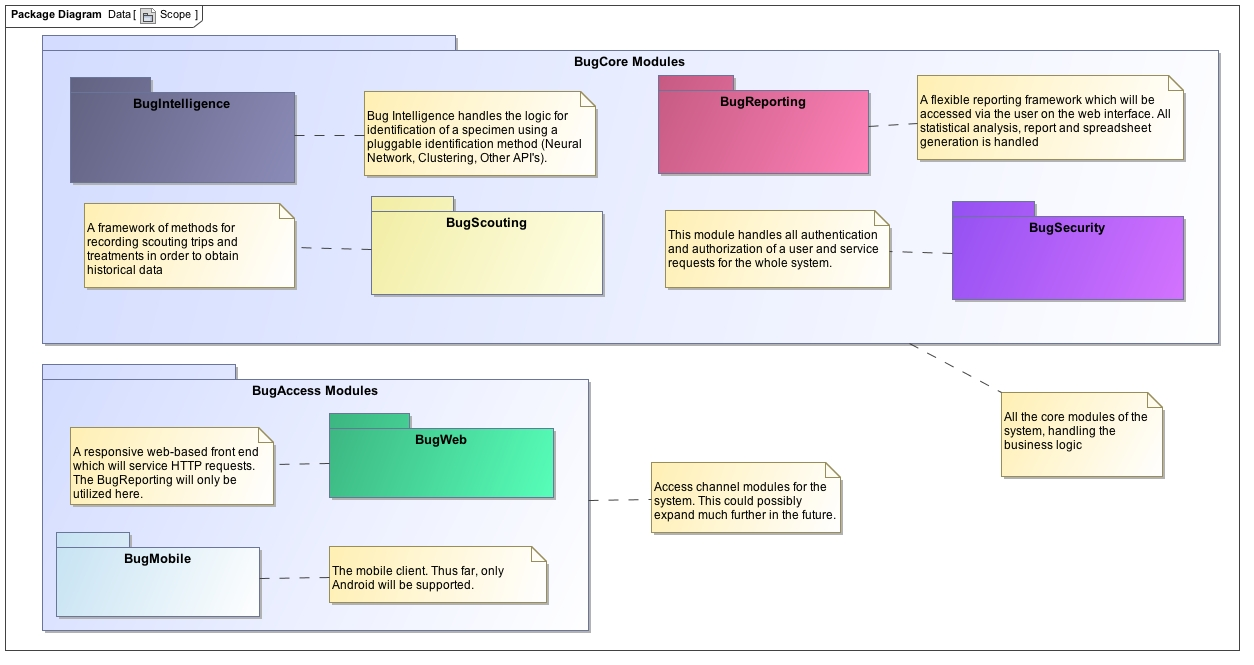
\includegraphics[width=\linewidth]{scope}

%\section{Architecture requirements}
%	\subsection{Access channel requirements}
%	\subsection{Quality requirements}
%	\subsection{Integration requirements}
%	\subsection{Architecture constraints}
\section{Functional Requirements and Application Design}
	\subsection{Domain Model}
	
%------------------------------------------------------------------------------------------%

	\subsection{BugScouting}
		The BugScouting module has the following functionality:
		\begin{enumerate}
			\item It provides the functionality for a user to be able to enter data related to a scouting trip - entering data such as the number of trees scouted, the average number of bugs per tree and the different kind of bugs specified. After which a summary should be displayed.
			\item It provides the ability for a user to record the details related to spraying.
		\end{enumerate}
		\subsubsection{Module Scope}
		The scope of the \textit{BugScouting} module is shown below:\\
		\hfill\\
		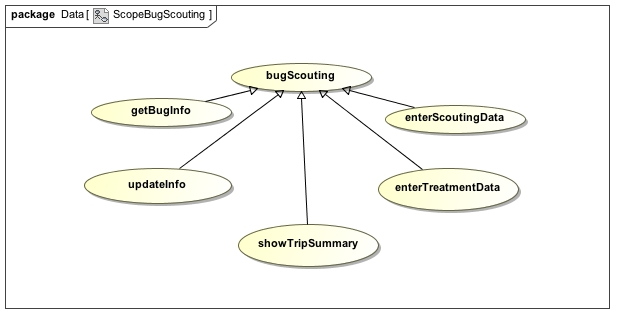
\includegraphics[width=\linewidth]{ScopeBugScouting}
		
		\subsubsection{Use Cases}
		The concrete use cases for the \textit{BugScouting} module follow:
		\paragraph{getBugInfo \dotfill [Priority - Medium]}
		This use case uses the BugIntelligence module to retrieve information on a specific specimen which will be used to display to the user a "wiki" like piece which has the purpose of informing the user.\\\hfill\\
		The Service Contract for the \textit{getBugInfo} use case is shown below:\\\hfill\\
		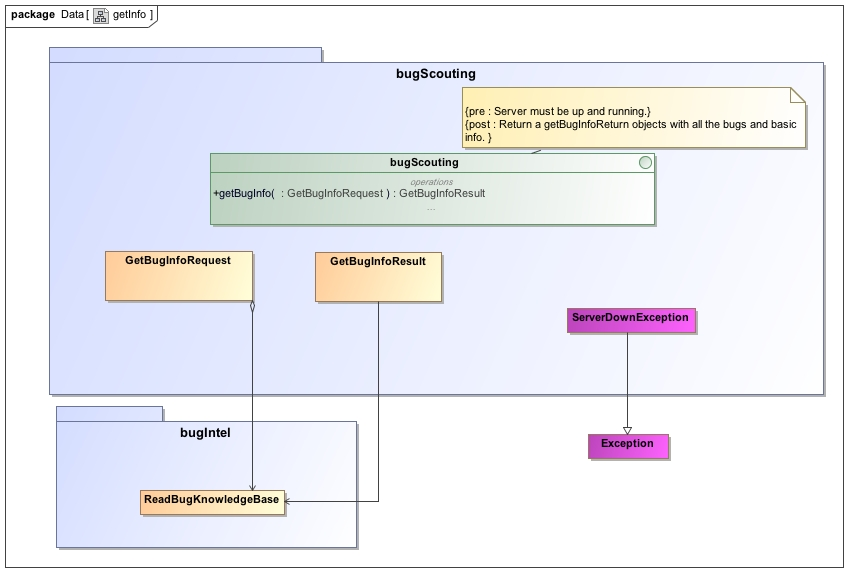
\includegraphics[width=\linewidth]{getInfo}
		
		\paragraph{updateInfo \dotfill [Priority - Medium]}
		The objective of this use case is to provide functionality to retrieve updated bug information and identification method updates.\\\hfill\\
		The Service Contract for the \textit{getBugInfo} use case is shown below:\\\hfill\\
		\includegraphics[width=\linewidth]{updateInfo}
		
		\paragraph{showTripSummary \dotfill [Priority - High]}
		After completing a full scouting trip, this use case should provide a summary of the entire scouting trip. One scouting trip may consist of many scouting stops. The averages for the scouting trip data is used in the summary.\\\hfill\\
		The Service Contract for the \textit{showTripSummary} use case is shown below:\\\hfill\\
		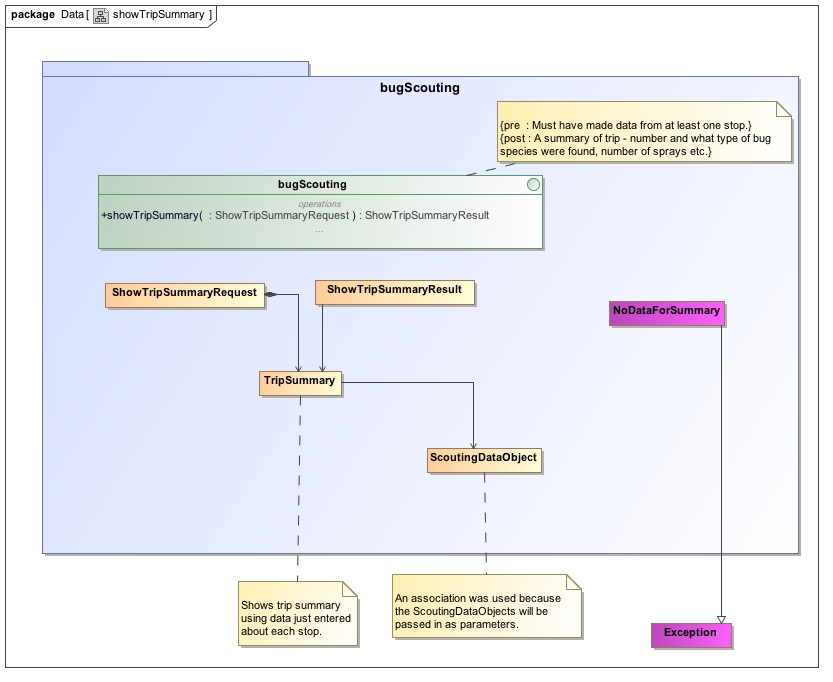
\includegraphics[width=\linewidth]{showTripSummary}
		
		\paragraph{enterTreatmentData \dotfill [Priority - Critical]}
		This use case is for entering data related to spraying chemicals (pesticide). This allows for the type of chemical, the date and the block or orchard number to be recorded.\\\hfill\\
		
		The Service Contract for the \textit{enterTreatmentData} use case is shown below:\\\hfill\\
		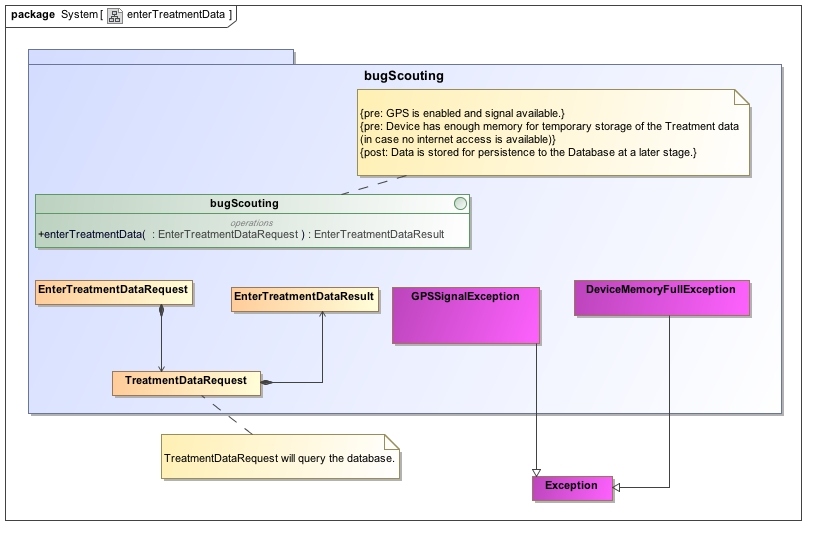
\includegraphics[width=\linewidth]{EnterTreatmentData}
		
		\paragraph{enterScoutingData \dotfill [Priority - Critical]}
		This is the core use case of this module. This use case allows entering data related to a scouting stop. Data captured should include the number of trees observed, number of bugs counter and the block or orchard number where the scouting took place. After entering the data, the specimen should be identified (classified) before successfully submitting it for persistence.\\\hfill\\
		The Service Contract for the \textit{enterScoutingData} use case is shown below:\\\hfill\\
		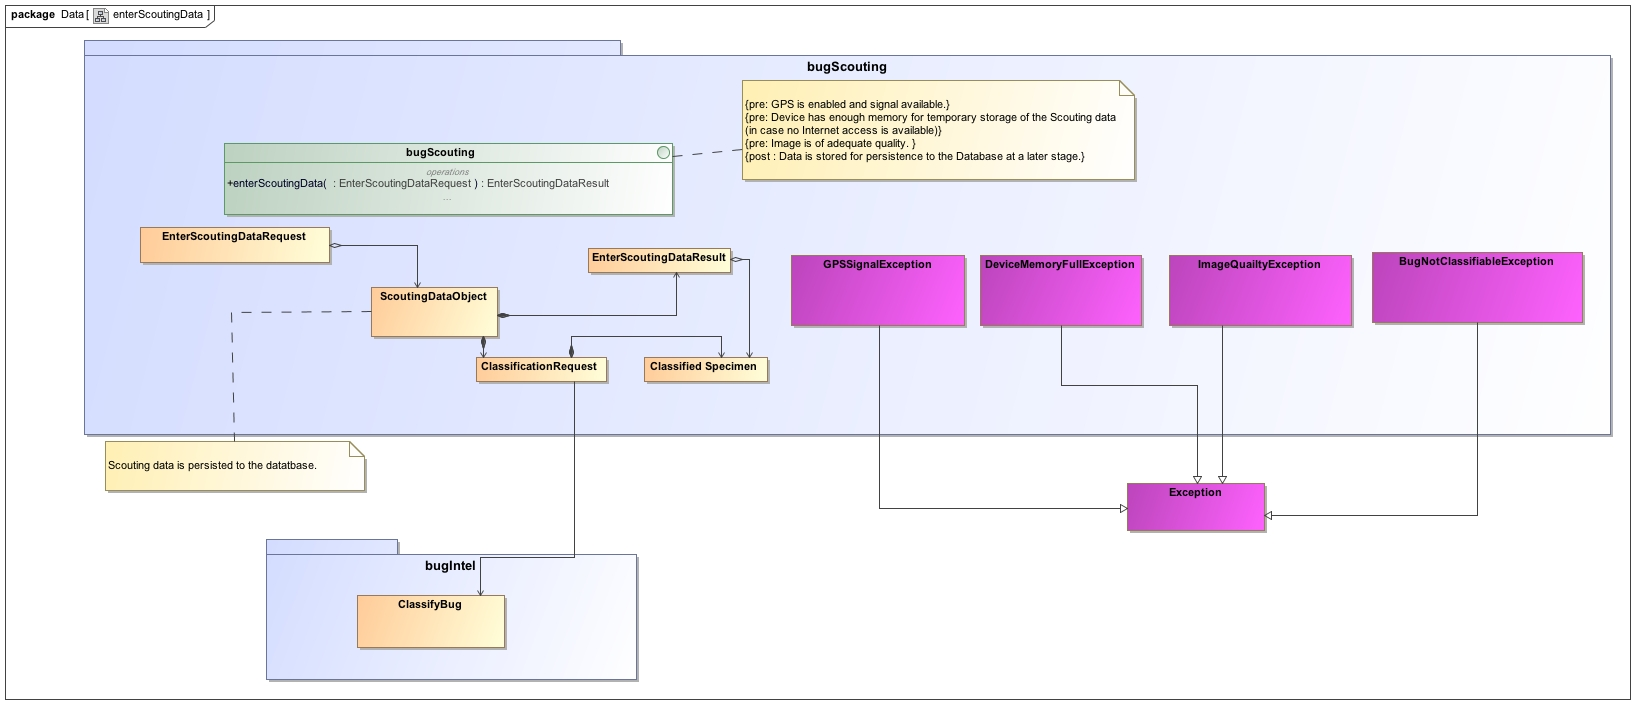
\includegraphics[width=\linewidth]{enterScoutingData}
		The Process Specification for the \textit{enterScoutingData} use case is shown below:\\\hfill\\
		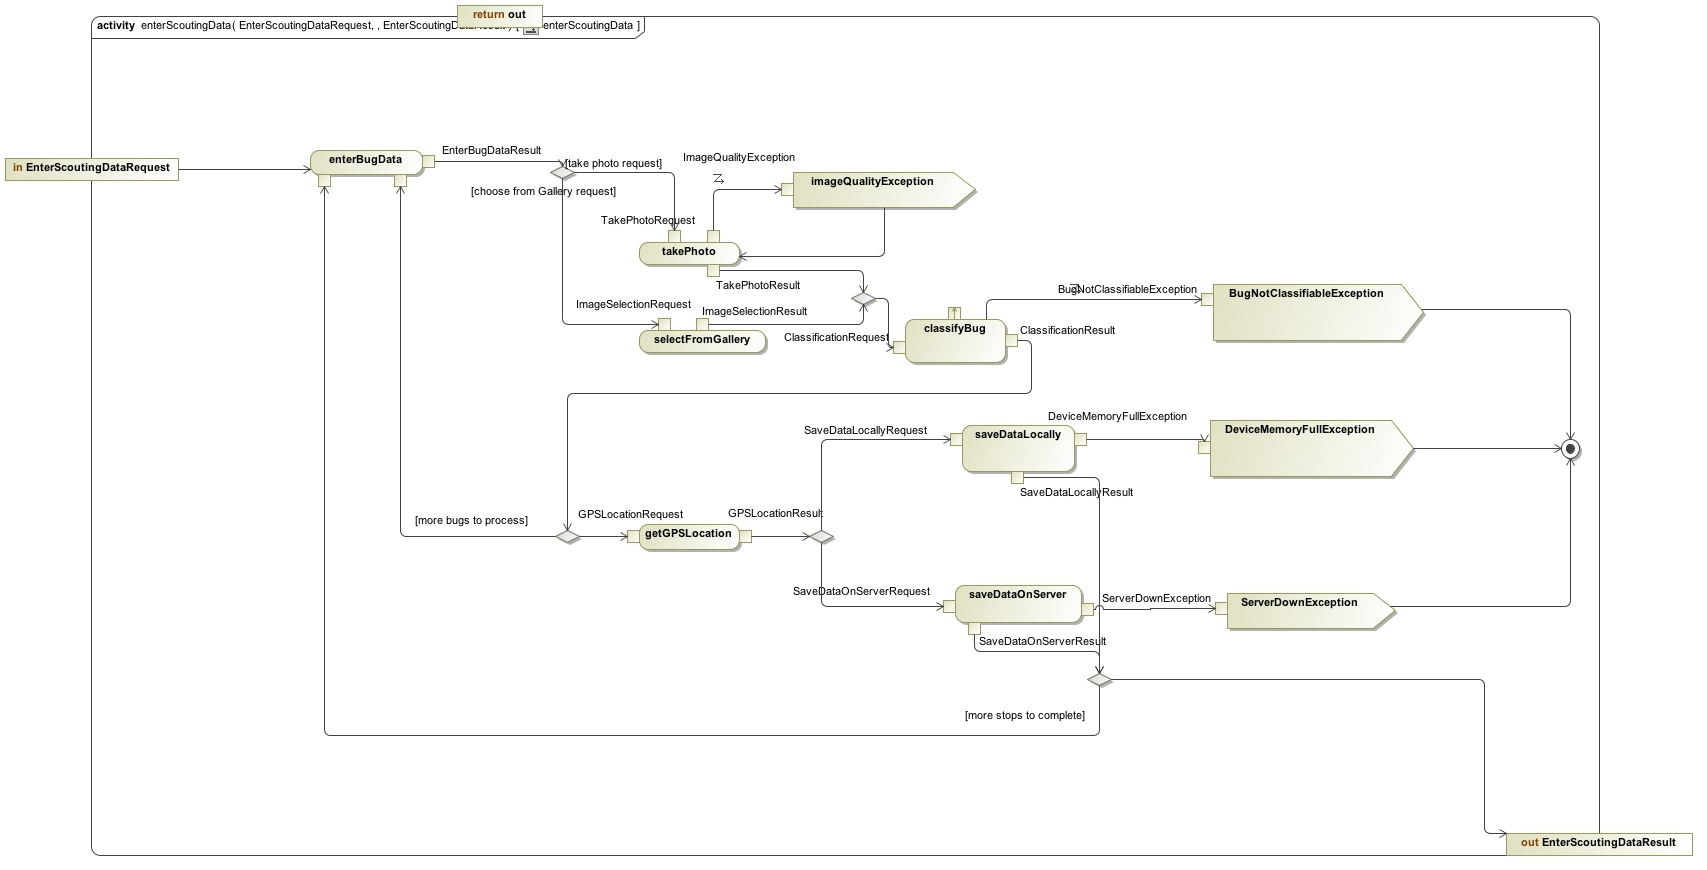
\includegraphics[width=\linewidth]{enterScoutingDataPS}
		
		
		
		
%------------------------------------------------------------------------------------------%	
	
	\subsection{BugIntelligence}
		The BugIntelligence module has the following functionality:
		\begin{enumerate}		
			\item It provides a pluggable method to classify a specimen according to species and life stage.
			\item It provides an interface which can be used to obtain information related to any specific specimen which is identifiable by the system
			\item It provides CRUD(Create Read Update Delete) functionality for bug information for specimens identifiable by the identification method
		\end{enumerate}
		\subsubsection{Module Scope}
		The scope of the \textit{BugIntelligence} module is shown below:\\
		\hfill\\
		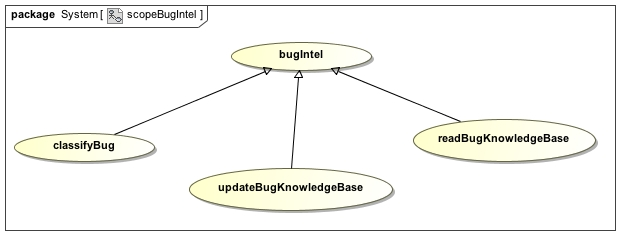
\includegraphics[width=\linewidth]{scopeBugIntel}
		\subsubsection{Use Cases}
		The concrete use cases for the \textit{BugIntelligence} module follow:
		
		\paragraph{classifyBug \dotfill [Priority - Critical]}
		This use case supplies a method to classify the bug according to life stage and species. The classification method used is pluggable.\\\hfill\\
		The Service Contract for the \textit{classifyBug} use case is shown below:\\\hfill\\
		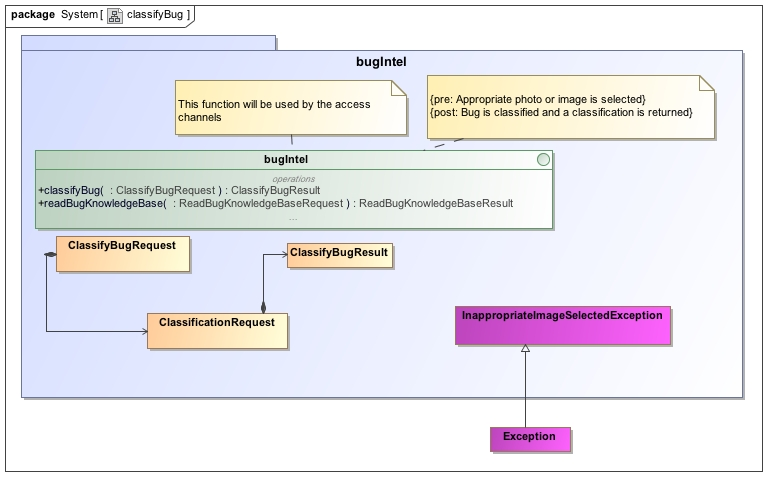
\includegraphics[width=\linewidth]{classifyBug}
		
		The Process Specification for the \textit{classifyBug} use case is shown below:\\\hfill\\
		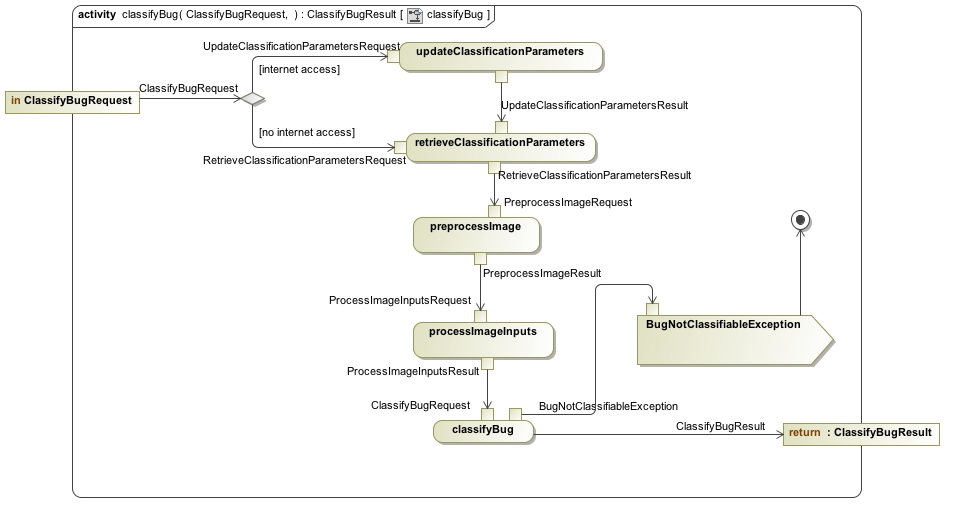
\includegraphics[width=\linewidth]{classfyBugPS}
		
		\paragraph{updateBugKnowledgeBase \dotfill [Priority - Low]}		
		This use case provides the functionality to edit the information used for classification. As in the example of a neural network being used as a classification method, the training examples may be edited.		
		The Service Contract for the \textit{updateBugKnowledgeBase} use case is shown below:\\\hfill\\
		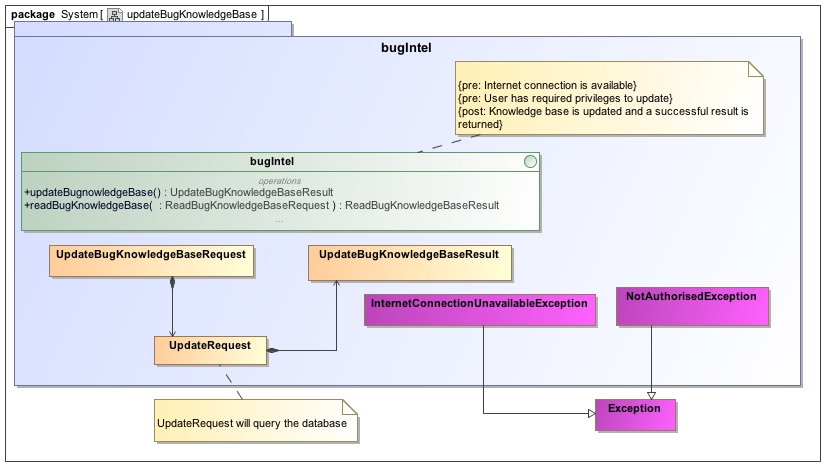
\includegraphics[width=\linewidth]{updateBugKnowledgeBase}
		
		\paragraph{readBugKnowledgeBase \dotfill [Priority - Critical]}
				This use case provides the functionality to get the information used for classification. As in the example of a neural network being used as a classification method, the training examples may be retrieved.	
		The Service Contract for the \textit{readBugKnowledgeBase} use case is shown below:\\\hfill\\
		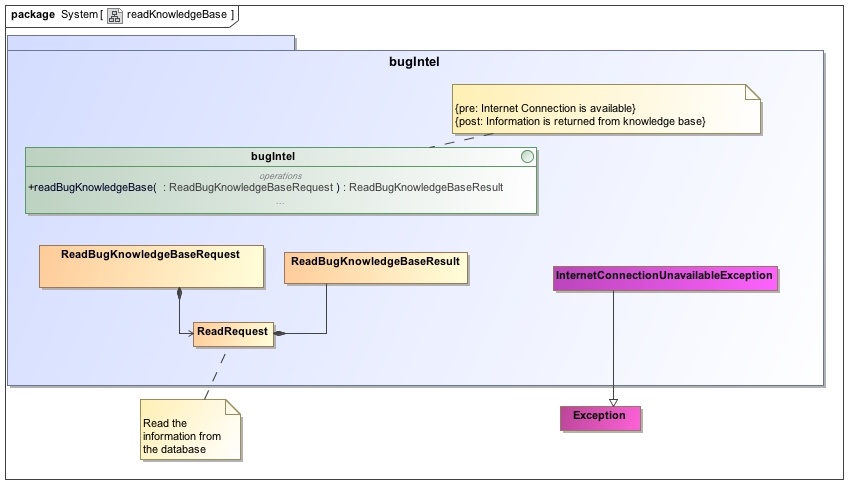
\includegraphics[width=\linewidth]{readKnowledgeBase}
		
		
%------------------------------------------------------------------------------------------%		
	\subsection{BugSecurity}
	The BugSecurity module allows the following functionality:
	\begin{enumerate}
		\item It provides functionality related to user accounts and user roles in order to login, register and recover your account within the capacity of a user role.
		\item It provides functionality to determine whether a specific service request should be allowed.
	\end{enumerate}
		\subsubsection{Module Scope}
		The scope of the \textit{BugSecurity} module is shown below:\\
		\hfill\\
		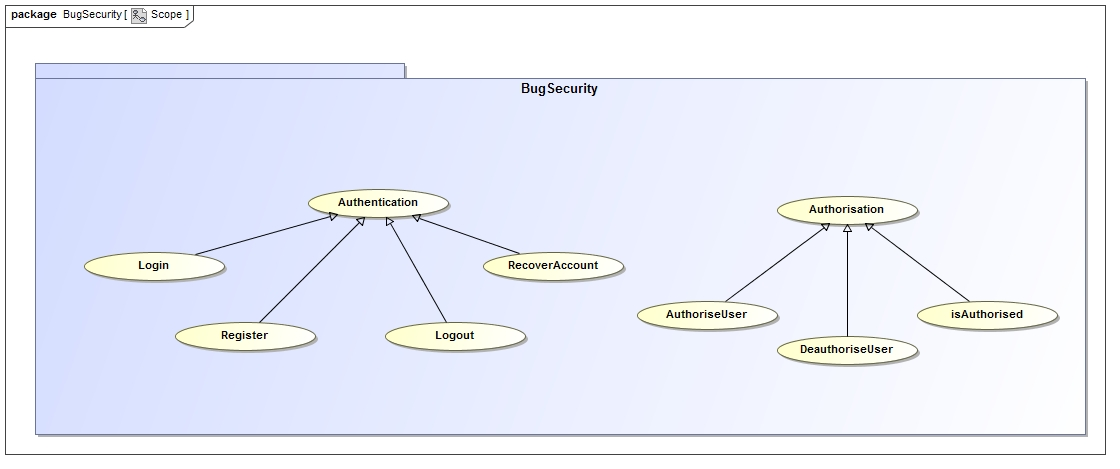
\includegraphics[width=\linewidth]{SecurityScope}
		\subsubsection{Use Cases}
		The concrete use cases for the \textit{BugSecurity} module follow:
		
		\paragraph{login \dotfill [Priority - Critical]}
		This use cases allows one to login with username and password credentials which will be validated and thus allowing the user to be authenticated.\\\hfill\\
		The Service Contract for the \textit{login} use case is shown below:\\\hfill\\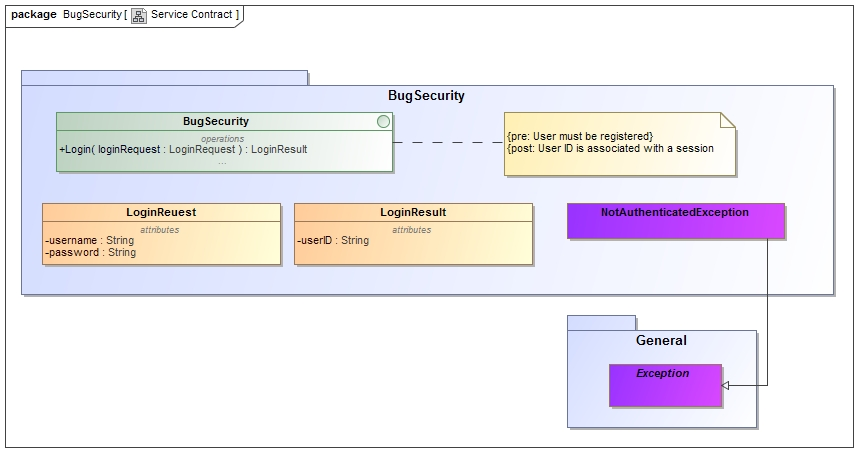
\includegraphics[width=\linewidth]{LoginSC}
		
		\paragraph{register \dotfill [Priority - Critical]}
		This use case caters for registration as a new user. A user account is created which is associated with a unique user name. Currently, there are no password format requirements.\\\hfill\\
		The Service Contract for the \textit{register} use case is shown below:\\\hfill\\
		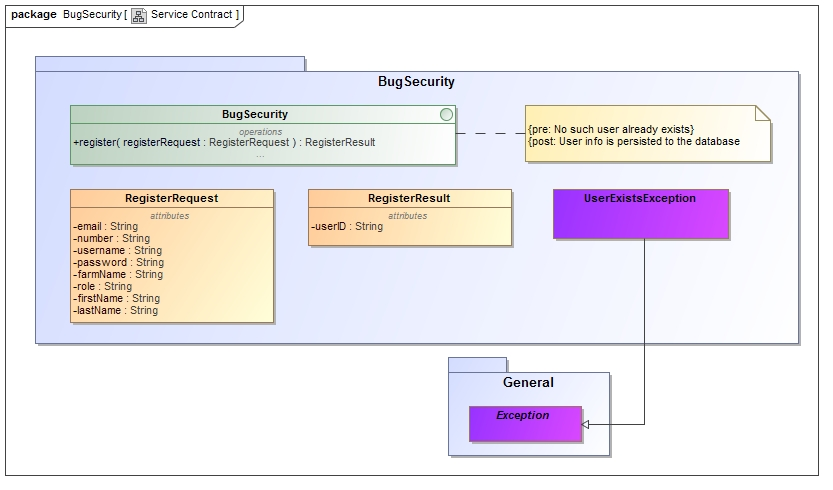
\includegraphics[width=\linewidth]{RegisterSC}		
		
		\paragraph{logout \dotfill [Priority - Medium]}
		This use case provides functionality to log out of the system.\\\hfill\\
		The Service Contract for the \textit{logout} use case is shown below:\\\hfill\\
		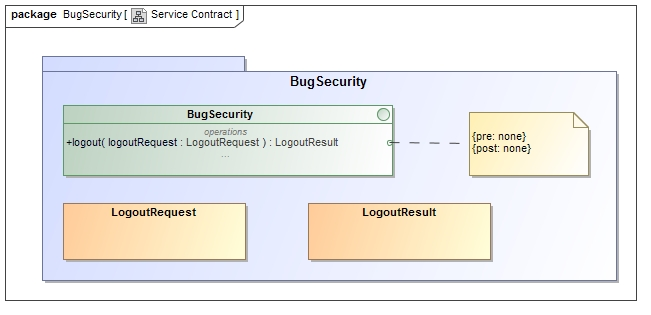
\includegraphics[width=\linewidth]{LogoutSC}
		
		\paragraph{recoverAccount \dotfill [Priority - Low]}
		In the case where a user forgets or has lost his/her credentials to access the system, this use case provides functionality to recover or to generate a new password. User verification is done via the email address associated with the account.\\\hfill\\ 
		The Service Contract for the \textit{recoverAccount} use case is shown below:\\\hfill\\
		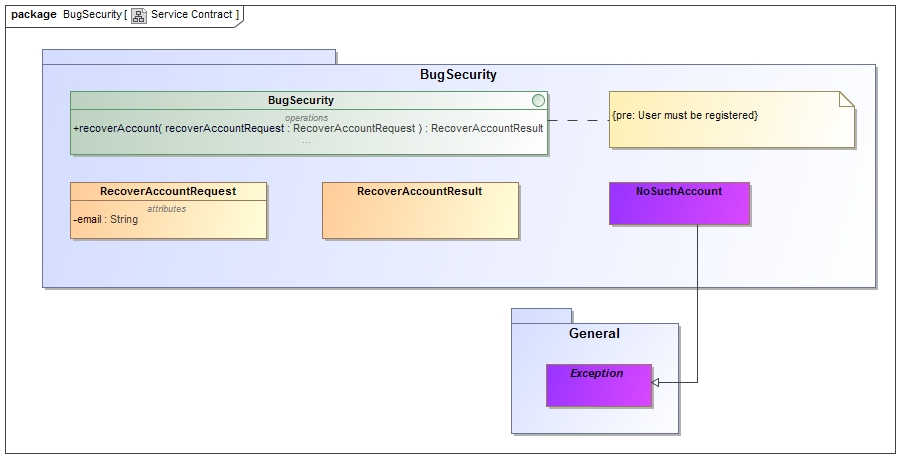
\includegraphics[width=\linewidth]{RecoverAccountSC}
		
		\paragraph{isAuthorised \dotfill [Priority - High]}
		Whenever a service which should not be accessibility to entire plethora of users is requested, authorization is required. This use case makes provision for this.\\\hfill\\
		The Service Contract for the \textit{isAuthorised} use case is shown below:\\\hfill\\
		%\includegraphics[width=\linewidth]{}
		\paragraph{authoriseUser \dotfill [Priority - Medium]}
		This use case allows for an authorization restriction for a service to be added/\\\hfill\\
		The Service Contract for the \textit{authoriseUser} use case is shown below:\\\hfill\\
		%\includegraphics[width=\linewidth]{}
		\paragraph{deauthoriseUser \dotfill [Priority - Medium]}
				This use case allows for an authorization restriction for a service to be removed/\\\hfill\\
		The Service Contract for the \textit{deauthoriseUser} use case is shown below:\\\hfill\\
		%\includegraphics[width=\linewidth]{}
		
		
		
%------------------------------------------------------------------------------------------%		
	\subsection{BugReporting}
	The BugReporting module allows the following functionality:
	\begin{enumerate}
		\item It provides functionality to generate historical data in a usable, tabular - as used by Microsoft Excel and similar software, format.
		\item It provides functionality to generate a visual representation of historical data in the form of a dynamically chosen set of graphs.
		\item It provides functionality to generate a heat map of the farm with regards to the population of stink bugs identified.
	\end{enumerate}
		\subsubsection{Module Scope}
		The scope of the \textit{BugReporting} module is shown below:\\
		\hfill\\
			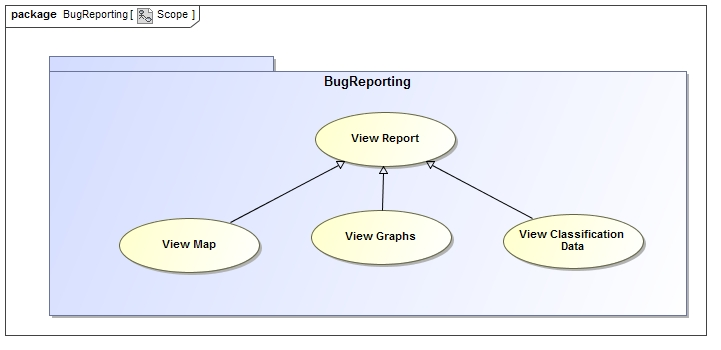
\includegraphics[width=\linewidth]{ReportingScope}
		\subsubsection{Use Cases}
		The concrete use cases for the \textit{BugReporting} module follow:
		\paragraph{viewMap \dotfill [Priority - Medium]}
		This use case allows for the generation of a heat map based on historical data.\\\hfill\\
		The Service Contract for the \textit{viewMap} use case is shown below:\\\hfill\\		
		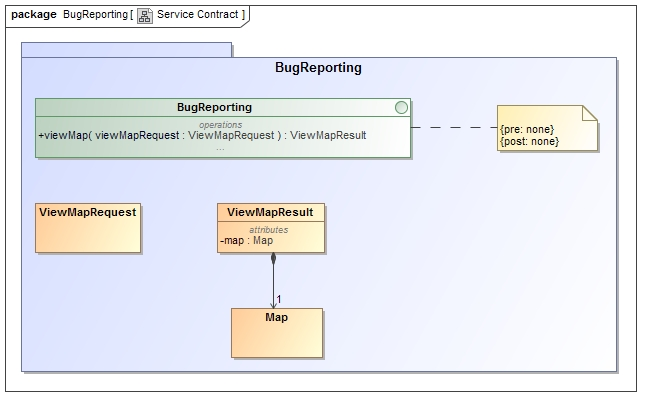
\includegraphics[width=\linewidth]{viewMapSC}
		
		\paragraph{viewGraph \dotfill [Priority - Medium]}
		This use case allows for the generation of a graphs based on historical data.\\\hfill\\
		The Service Contract for the \textit{viewGraph} use case is shown below:\\\hfill\\	
		\includegraphics[width=\linewidth]{viewGraphSC}	
		
		\paragraph{viewHistoricalData \dotfill [Priority - Medium]}
		This use case allows for the generation of historical data.\\\hfill\\
		The Service Contract for the \textit{viewHistoricalData} use case is shown below:\\\hfill\\
				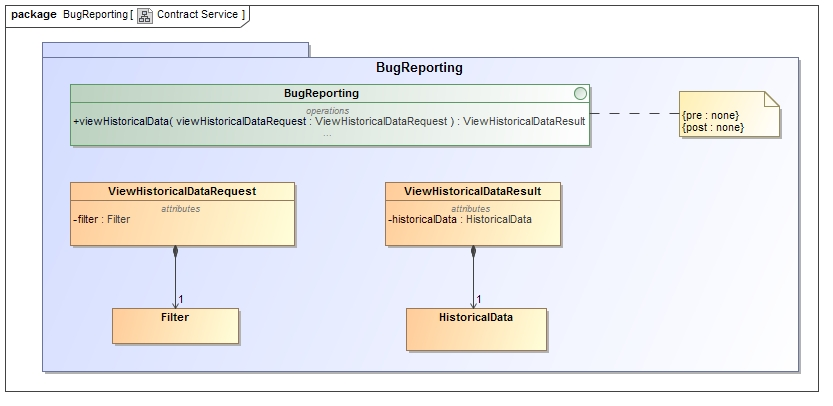
\includegraphics[width=\linewidth]{viewHistoricalDataSC}	

	
		
		
\section{Architectural Requirements}
	\subsection{Quality Requirements}
		\subsubsection{Maintainability}
			As a standard requirement for all projects, SAMBUG needs to be maintainable. This is especially due to the fact that the project has very high expansion potential. SUBTROP has shown interest in further maintaining the project after completion.
		\subsubsection{Scalability}
			Since the user base for the system will be comparatively small, scalability is not a great issue. The load on the system will not under any foreseeable circumstances be extremely high.
		\subsubsection{Performance Requirements}
			Performance is a very important requirement for the system. The goal of the system is to provide an efficient service rendered. Users of the system will be subject to high pressure environments where time is an issue.
		\subsubsection{Reliability and Availability}
			Since users will be relying heavily on this system to make important business decisions the system must be available to be used at all times. As such, a reliable system is of paramount importance.
		\subsubsection{Security}
			As specified by the client, for the sake of reducing usage complexity of the system, the security may be relaxed in this case due to the fact that the users are generally not comfortable with using technological products.
		\subsubsection{Auditability}
			There is no specific auditability requirement for the system since there will be no business value in tracking user activity.
		\subsubsection{Testability}
			Every service offered by the system should be testable via:\\
			1. Unit tests\\
			2. Integration tests
		\subsubsection{Usability}
			Usability is the main quality requirement for the system. In order for the system to have any actual business value it should be easy to use and effective.
		\subsubsection{Deployability}
			The system must be deployable to any cloud hosted virtual machine or locally hosted server.
	\subsection{Architecture responsibilities}
	The architectural responsibilities of the system include providing infrastructure for the following:
		\begin{itemize}
			\item A web access channel
			\item A mobile access channel
			\item Hosting for business logic and services offered by the system
			\item Relational database persistence
			\item Sending emails for recovering of accounts
		\end{itemize}
\section{Architectural Design}
	\subsection{Overview}
		A layered architecture will be used with the following layers:
			\begin{itemize}
				\item Access Layer
					\begin{itemize}
						\item 
					\end{itemize}
				\item Services Layer
				\item Data Access Layer
			\end{itemize}
	\subsection{Infrastructure Layout}
		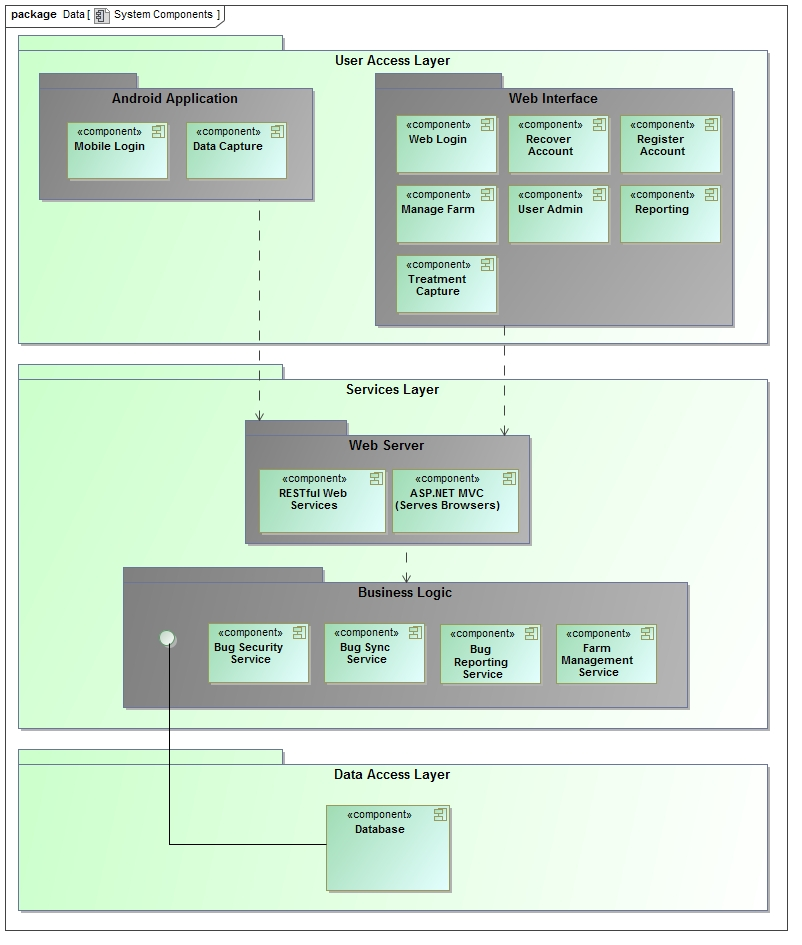
\includegraphics[width=\linewidth]{SystemComponents}	
	\subsection{Database Design}
	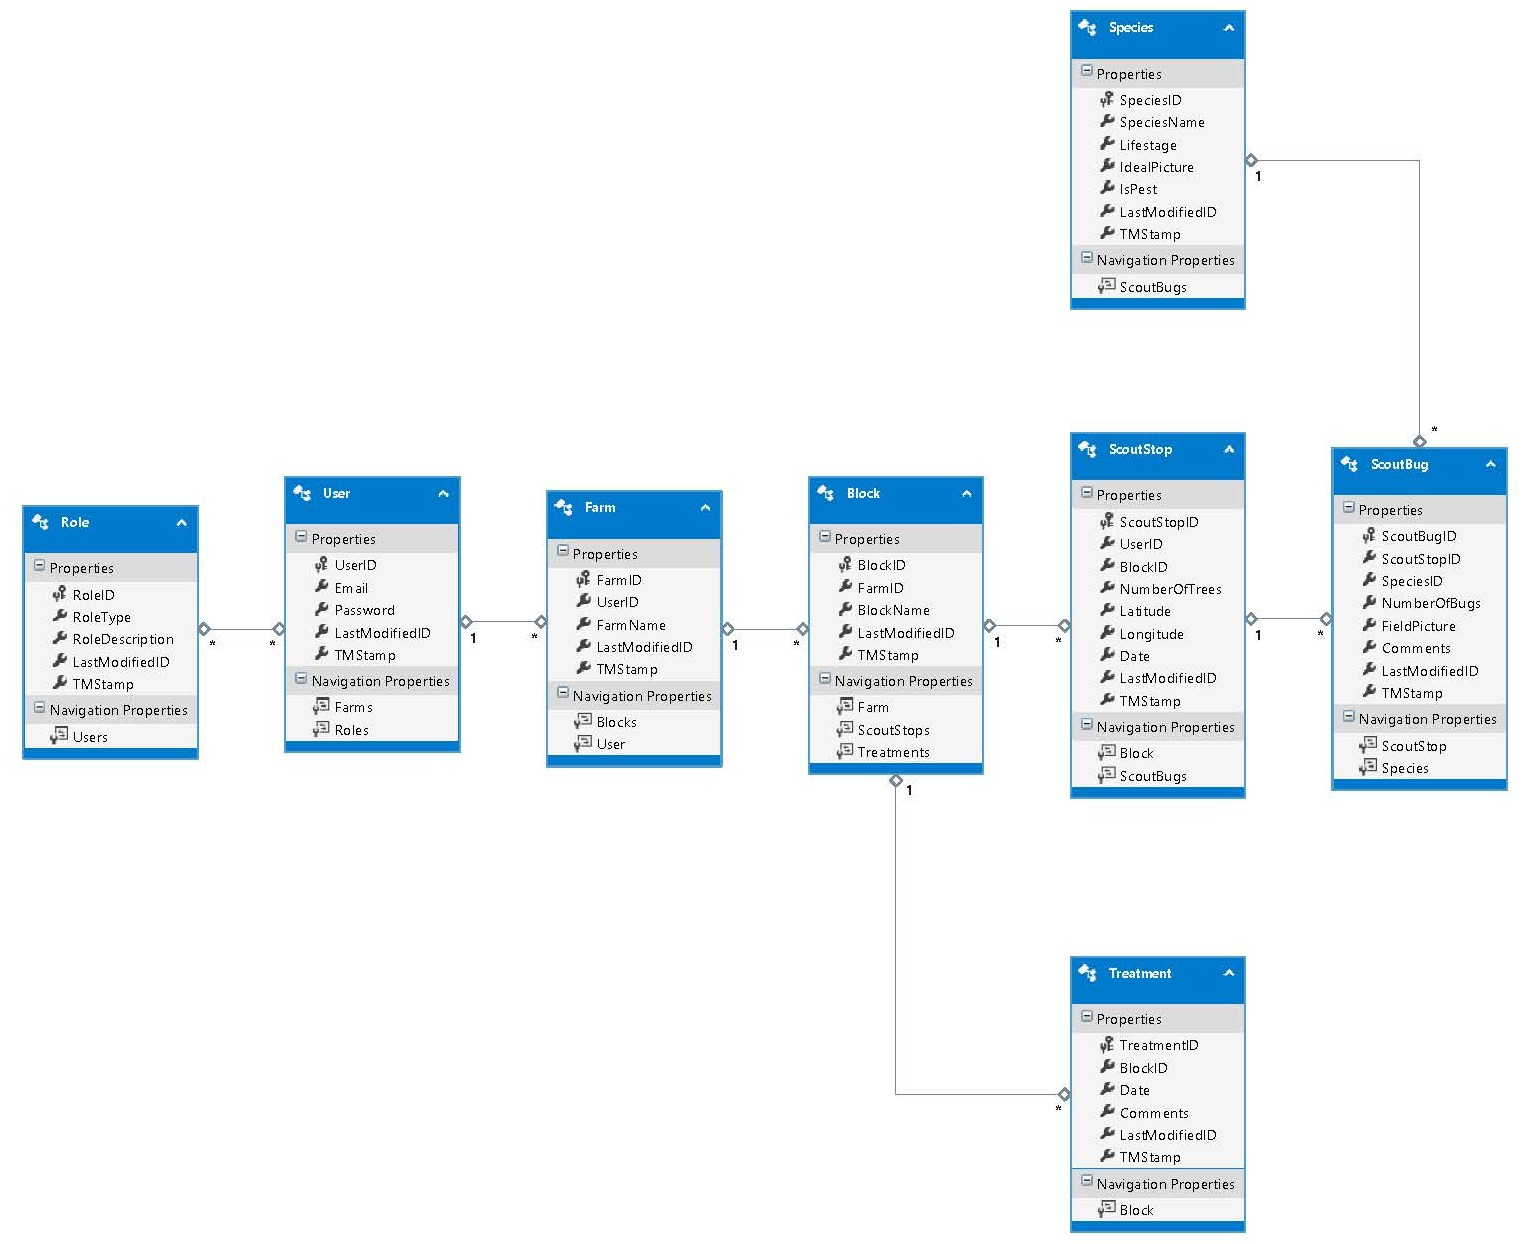
\includegraphics[width=\linewidth]{ERD}	
	\subsection{Process Flow}
		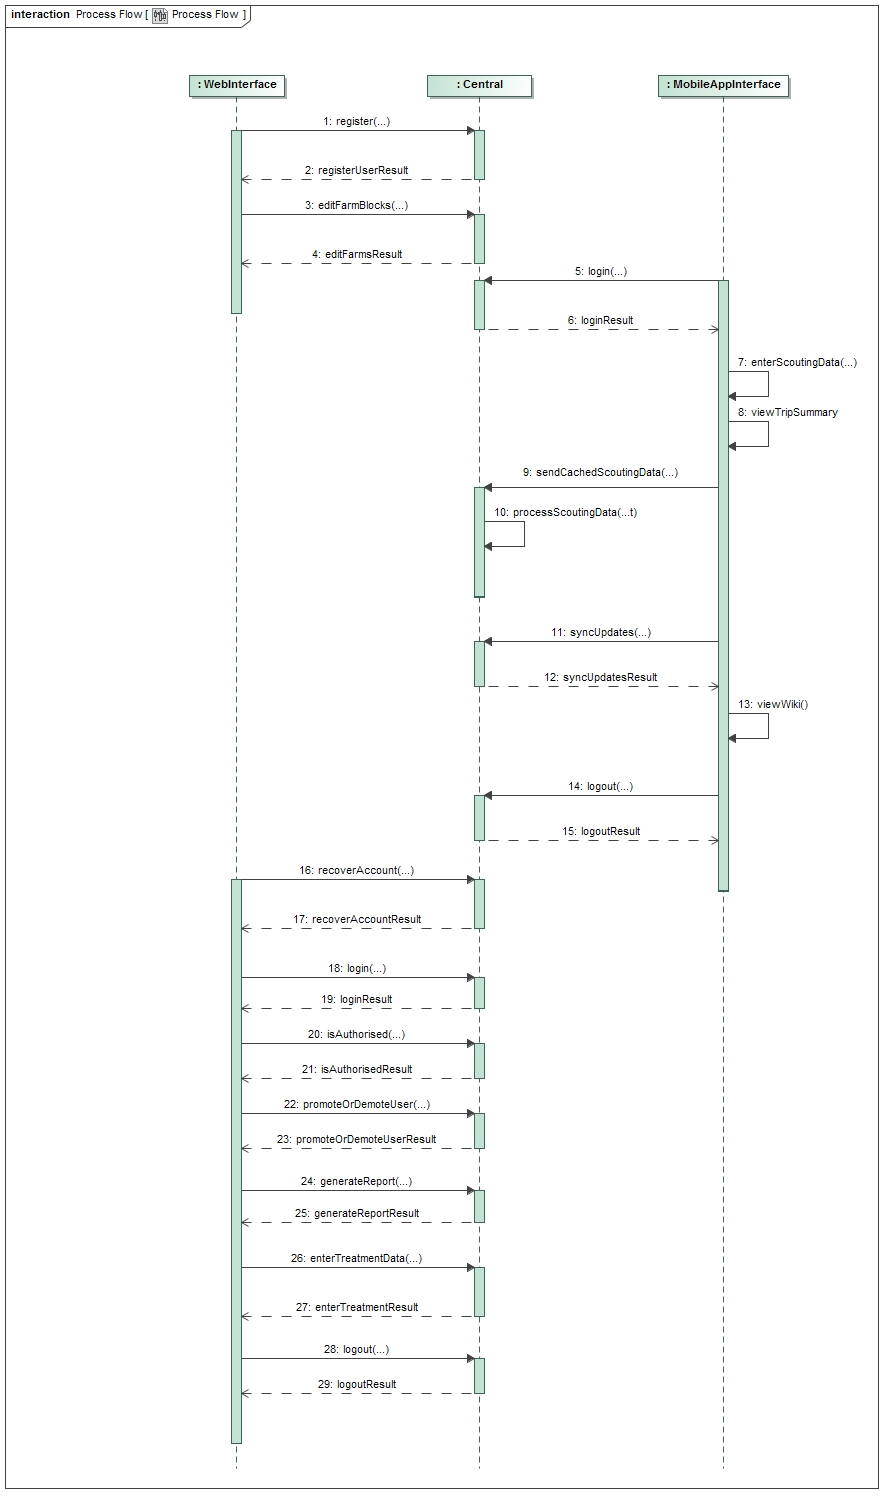
\includegraphics[width=\linewidth]{ProcessFlow}	
	\subsection{Technologies}
		\subsubsection{Mobile Application}
			\paragraph{Android Studio}
		\subsubsection{Web Backend}
			\paragraph{.NET REST Services}
			\paragraph{SQL Server}
		\subsubsection{Web Frontend}
			\paragraph{Aurelia.io}
		\subsubsection{Builds}		
			\paragraph{TeamCity}
			\paragraph{Gradle}
			\paragraph{MSBuild}
		\subsubsection{Testing}
			\paragraph{JUnit}
			\paragraph{NUnit}
	
	

%\section{Open Issues}


%\pagebreak
%\section{Notifications and Messages Domain}
%  \input{Notifications}

\end{document}